
%% bare_conf.tex
%% V1.3
%% 2007/01/11
%% by Michael Shell
%% See:
%% http://www.michaelshell.org/
%% for current contact information.
%%
%% This is a skeleton file demonstrating the use of IEEEtran.cls
%% (requires IEEEtran.cls version 1.7 or later) with an IEEE conference paper.
%%
%% Support sites:
%% http://www.michaelshell.org/tex/ieeetran/
%% http://www.ctan.org/tex-archive/macros/latex/contrib/IEEEtran/
%% and
%% http://www.ieee.org/

%%*************************************************************************
%% Legal Notice:
%% This code is offered as-is without any warranty either expressed or
%% implied; without even the implied warranty of MERCHANTABILITY or
%% FITNESS FOR A PARTICULAR PURPOSE! 
%% User assumes all risk.
%% In no event shall IEEE or any contributor to this code be liable for
%% any damages or losses, including, but not limited to, incidental,
%% consequential, or any other damages, resulting from the use or misuse
%% of any information contained here.
%%
%% All comments are the opinions of their respective authors and are not
%% necessarily endorsed by the IEEE.
%%
%% This work is distributed under the LaTeX Project Public License (LPPL)
%% ( http://www.latex-project.org/ ) version 1.3, and may be freely used,
%% distributed and modified. A copy of the LPPL, version 1.3, is included
%% in the base LaTeX documentation of all distributions of LaTeX released
%% 2003/12/01 or later.
%% Retain all contribution notices and credits.
%% ** Modified files should be clearly indicated as such, including  **
%% ** renaming them and changing author support contact information. **
%%
%% File list of work: IEEEtran.cls, IEEEtran_HOWTO.pdf, bare_adv.tex,
%%                    bare_conf.tex, bare_jrnl.tex, bare_jrnl_compsoc.tex
%%*************************************************************************

% *** Authors should verify (and, if needed, correct) their LaTeX system  ***
% *** with the testflow diagnostic prior to trusting their LaTeX platform ***
% *** with production work. IEEE's font choices can trigger bugs that do  ***
% *** not appear when using other class files.                            ***
% The testflow support page is at:
% http://www.michaelshell.org/tex/testflow/



% Note that the a4paper option is mainly intended so that authors in
% countries using A4 can easily print to A4 and see how their papers will
% look in print - the typesetting of the document will not typically be
% affected with changes in paper size (but the bottom and side margins will).
% Use the testflow package mentioned above to verify correct handling of
% both paper sizes by the user's LaTeX system.
%
% Also note that the "draftcls" or "draftclsnofoot", not "draft", option
% should be used if it is desired that the figures are to be displayed in
% draft mode.
%
\documentclass[conference]{IEEEtran}
% Add the compsoc option for Computer Society conferences.
%
% If IEEEtran.cls has not been installed into the LaTeX system files,
% manually specify the path to it like:
% \documentclass[conference]{../sty/IEEEtran}
\usepackage{booktabs}       % professional-quality tables
\usepackage{color}
\usepackage{graphicx}
\usepackage{subfigure}
\usepackage{comment}
\usepackage[fleqn]{amsmath}
\usepackage{multirow}
\usepackage{comment}
% Some very useful LaTeX packages include:
% (uncomment the ones you want to load)


% *** MISC UTILITY PACKAGES ***
%
%\usepackage{ifpdf}
% Heiko Oberdiek's ifpdf.sty is very useful if you need conditional
% compilation based on whether the output is pdf or dvi.
% usage:
% \ifpdf
%   % pdf code
% \else
%   % dvi code
% \fi
% The latest version of ifpdf.sty can be obtained from:
% http://www.ctan.org/tex-archive/macros/latex/contrib/oberdiek/
% Also, note that IEEEtran.cls V1.7 and later provides a builtin
% \ifCLASSINFOpdf conditional that works the same way.
% When switching from latex to pdflatex and vice-versa, the compiler may
% have to be run twice to clear warning/error messages.






% *** CITATION PACKAGES ***
%
%\usepackage{cite}
% cite.sty was written by Donald Arseneau
% V1.6 and later of IEEEtran pre-defines the format of the cite.sty package
% \cite{} output to follow that of IEEE. Loading the cite package will
% result in citation numbers being automatically sorted and properly
% "compressed/ranged". e.g., [1], [9], [2], [7], [5], [6] without using
% cite.sty will become [1], [2], [5]--[7], [9] using cite.sty. cite.sty's
% \cite will automatically add leading space, if needed. Use cite.sty's
% noadjust option (cite.sty V3.8 and later) if you want to turn this off.
% cite.sty is already installed on most LaTeX systems. Be sure and use
% version 4.0 (2003-05-27) and later if using hyperref.sty. cite.sty does
% not currently provide for hyperlinked citations.
% The latest version can be obtained at:
% http://www.ctan.org/tex-archive/macros/latex/contrib/cite/
% The documentation is contained in the cite.sty file itself.






% *** GRAPHICS RELATED PACKAGES ***
%
\ifCLASSINFOpdf
  % \usepackage[pdftex]{graphicx}
  % declare the path(s) where your graphic files are
  % \graphicspath{{../pdf/}{../jpeg/}}
  % and their extensions so you won't have to specify these with
  % every instance of \includegraphics
  % \DeclareGraphicsExtensions{.pdf,.jpeg,.png}
\else
  % or other class option (dvipsone, dvipdf, if not using dvips). graphicx
  % will default to the driver specified in the system graphics.cfg if no
  % driver is specified.
  % \usepackage[dvips]{graphicx}
  % declare the path(s) where your graphic files are
  % \graphicspath{{../eps/}}
  % and their extensions so you won't have to specify these with
  % every instance of \includegraphics
  % \DeclareGraphicsExtensions{.eps}
\fi
% graphicx was written by David Carlisle and Sebastian Rahtz. It is
% required if you want graphics, photos, etc. graphicx.sty is already
% installed on most LaTeX systems. The latest version and documentation can
% be obtained at: 
% http://www.ctan.org/tex-archive/macros/latex/required/graphics/
% Another good source of documentation is "Using Imported Graphics in
% LaTeX2e" by Keith Reckdahl which can be found as epslatex.ps or
% epslatex.pdf at: http://www.ctan.org/tex-archive/info/
%
% latex, and pdflatex in dvi mode, support graphics in encapsulated
% postscript (.eps) format. pdflatex in pdf mode supports graphics
% in .pdf, .jpeg, .png and .mps (metapost) formats. Users should ensure
% that all non-photo figures use a vector format (.eps, .pdf, .mps) and
% not a bitmapped formats (.jpeg, .png). IEEE frowns on bitmapped formats
% which can result in "jaggedy"/blurry rendering of lines and letters as
% well as large increases in file sizes.
%
% You can find documentation about the pdfTeX application at:
% http://www.tug.org/applications/pdftex





% *** MATH PACKAGES ***
%
%\usepackage[cmex10]{amsmath}
% A popular package from the American Mathematical Society that provides
% many useful and powerful commands for dealing with mathematics. If using
% it, be sure to load this package with the cmex10 option to ensure that
% only type 1 fonts will utilized at all point sizes. Without this option,
% it is possible that some math symbols, particularly those within
% footnotes, will be rendered in bitmap form which will result in a
% document that can not be IEEE Xplore compliant!
%
% Also, note that the amsmath package sets \interdisplaylinepenalty to 10000
% thus preventing page breaks from occurring within multiline equations. Use:
%\interdisplaylinepenalty=2500
% after loading amsmath to restore such page breaks as IEEEtran.cls normally
% does. amsmath.sty is already installed on most LaTeX systems. The latest
% version and documentation can be obtained at:
% http://www.ctan.org/tex-archive/macros/latex/required/amslatex/math/





% *** SPECIALIZED LIST PACKAGES ***
%
%\usepackage{algorithmic}
% algorithmic.sty was written by Peter Williams and Rogerio Brito.
% This package provides an algorithmic environment fo describing algorithms.
% You can use the algorithmic environment in-text or within a figure
% environment to provide for a floating algorithm. Do NOT use the algorithm
% floating environment provided by algorithm.sty (by the same authors) or
% algorithm2e.sty (by Christophe Fiorio) as IEEE does not use dedicated
% algorithm float types and packages that provide these will not provide
% correct IEEE style captions. The latest version and documentation of
% algorithmic.sty can be obtained at:
% http://www.ctan.org/tex-archive/macros/latex/contrib/algorithms/
% There is also a support site at:
% http://algorithms.berlios.de/index.html
% Also of interest may be the (relatively newer and more customizable)
% algorithmicx.sty package by Szasz Janos:
% http://www.ctan.org/tex-archive/macros/latex/contrib/algorithmicx/




% *** ALIGNMENT PACKAGES ***
%
%\usepackage{array}
% Frank Mittelbach's and David Carlisle's array.sty patches and improves
% the standard LaTeX2e array and tabular environments to provide better
% appearance and additional user controls. As the default LaTeX2e table
% generation code is lacking to the point of almost being broken with
% respect to the quality of the end results, all users are strongly
% advised to use an enhanced (at the very least that provided by array.sty)
% set of table tools. array.sty is already installed on most systems. The
% latest version and documentation can be obtained at:
% http://www.ctan.org/tex-archive/macros/latex/required/tools/


%\usepackage{mdwmath}
%\usepackage{mdwtab}
% Also highly recommended is Mark Wooding's extremely powerful MDW tools,
% especially mdwmath.sty and mdwtab.sty which are used to format equations
% and tables, respectively. The MDWtools set is already installed on most
% LaTeX systems. The lastest version and documentation is available at:
% http://www.ctan.org/tex-archive/macros/latex/contrib/mdwtools/


% IEEEtran contains the IEEEeqnarray family of commands that can be used to
% generate multiline equations as well as matrices, tables, etc., of high
% quality.


%\usepackage{eqparbox}
% Also of notable interest is Scott Pakin's eqparbox package for creating
% (automatically sized) equal width boxes - aka "natural width parboxes".
% Available at:
% http://www.ctan.org/tex-archive/macros/latex/contrib/eqparbox/





% *** SUBFIGURE PACKAGES ***
%\usepackage[tight,footnotesize]{subfigure}
% subfigure.sty was written by Steven Douglas Cochran. This package makes it
% easy to put subfigures in your figures. e.g., "Figure 1a and 1b". For IEEE
% work, it is a good idea to load it with the tight package option to reduce
% the amount of white space around the subfigures. subfigure.sty is already
% installed on most LaTeX systems. The latest version and documentation can
% be obtained at:
% http://www.ctan.org/tex-archive/obsolete/macros/latex/contrib/subfigure/
% subfigure.sty has been superceeded by subfig.sty.



%\usepackage[caption=false]{caption}
%\usepackage[font=footnotesize]{subfig}
% subfig.sty, also written by Steven Douglas Cochran, is the modern
% replacement for subfigure.sty. However, subfig.sty requires and
% automatically loads Axel Sommerfeldt's caption.sty which will override
% IEEEtran.cls handling of captions and this will result in nonIEEE style
% figure/table captions. To prevent this problem, be sure and preload
% caption.sty with its "caption=false" package option. This is will preserve
% IEEEtran.cls handing of captions. Version 1.3 (2005/06/28) and later 
% (recommended due to many improvements over 1.2) of subfig.sty supports
% the caption=false option directly:
%\usepackage[caption=false,font=footnotesize]{subfig}
%
% The latest version and documentation can be obtained at:
% http://www.ctan.org/tex-archive/macros/latex/contrib/subfig/
% The latest version and documentation of caption.sty can be obtained at:
% http://www.ctan.org/tex-archive/macros/latex/contrib/caption/




% *** FLOAT PACKAGES ***
%
%\usepackage{fixltx2e}
% fixltx2e, the successor to the earlier fix2col.sty, was written by
% Frank Mittelbach and David Carlisle. This package corrects a few problems
% in the LaTeX2e kernel, the most notable of which is that in current
% LaTeX2e releases, the ordering of single and double column floats is not
% guaranteed to be preserved. Thus, an unpatched LaTeX2e can allow a
% single column figure to be placed prior to an earlier double column
% figure. The latest version and documentation can be found at:
% http://www.ctan.org/tex-archive/macros/latex/base/



%\usepackage{stfloats}
% stfloats.sty was written by Sigitas Tolusis. This package gives LaTeX2e
% the ability to do double column floats at the bottom of the page as well
% as the top. (e.g., "\begin{figure*}[!b]" is not normally possible in
% LaTeX2e). It also provides a command:
%\fnbelowfloat
% to enable the placement of footnotes below bottom floats (the standard
% LaTeX2e kernel puts them above bottom floats). This is an invasive package
% which rewrites many portions of the LaTeX2e float routines. It may not work
% with other packages that modify the LaTeX2e float routines. The latest
% version and documentation can be obtained at:
% http://www.ctan.org/tex-archive/macros/latex/contrib/sttools/
% Documentation is contained in the stfloats.sty comments as well as in the
% presfull.pdf file. Do not use the stfloats baselinefloat ability as IEEE
% does not allow \baselineskip to stretch. Authors submitting work to the
% IEEE should note that IEEE rarely uses double column equations and
% that authors should try to avoid such use. Do not be tempted to use the
% cuted.sty or midfloat.sty packages (also by Sigitas Tolusis) as IEEE does
% not format its papers in such ways.





% *** PDF, URL AND HYPERLINK PACKAGES ***
%
%\usepackage{url}
% url.sty was written by Donald Arseneau. It provides better support for
% handling and breaking URLs. url.sty is already installed on most LaTeX
% systems. The latest version can be obtained at:
% http://www.ctan.org/tex-archive/macros/latex/contrib/misc/
% Read the url.sty source comments for usage information. Basically,
% \url{my_url_here}.





% *** Do not adjust lengths that control margins, column widths, etc. ***
% *** Do not use packages that alter fonts (such as pslatex).         ***
% There should be no need to do such things with IEEEtran.cls V1.6 and later.
% (Unless specifically asked to do so by the journal or conference you plan
% to submit to, of course. )


% correct bad hyphenation here
\hyphenation{op-tical net-works semi-conduc-tor}

\newcommand{\tabincell}[2]{\begin{tabular}{@{}#1@{}}#2\end{tabular}}

\begin{document}
%
% paper title
% can use linebreaks \\ within to get better formatting as desired
%\title{Deep convolutional neural network and data augamentation for fish detection and classifaction}
\title{Fish recognition using deep convolutional neural network and data augmentation}

% author names and affiliations
% use a multiple column layout for up to three different
% affiliations

\author{\IEEEauthorblockN{Ziqiang Zheng, Chao Wang, Zhibin Yu*, Haiyong Zheng, Weiwei Wang}
\IEEEauthorblockA{College of Information Science and Engineering\\
Ocean University of China\\
Qingdao 266100, China\\
Email: zhengziqiang1@gmail.com\\
*Corresponding author: yuzhibin@ouc.edu.cn}}


    % conference papers do not typically use \thanks and this command
% is locked out in conference mode. If really needed, such as for
% the acknowledgment of grants, issue a \IEEEoverridecommandlockouts
% after \documentclass

% for over three affiliations, or if they all won't fit within the width
% of the page, use this alternative format:
% 
%\author{\IEEEauthorblockN{Michael Shell\IEEEauthorrefmark{1},
%Homer Simpson\IEEEauthorrefmark{2},
%James Kirk\IEEEauthorrefmark{3}, 
%Montgomery Scott\IEEEauthorrefmark{3} and
%Eldon Tyrell\IEEEauthorrefmark{4}}
%\IEEEauthorblockA{\IEEEauthorrefmark{1}School of Electrical and Computer Engineering\\
%Georgia Institute of Technology,
%Atlanta, Georgia 30332--0250\\ Email: see http://www.michaelshell.org/contact.html}
%\IEEEauthorblockA{\IEEEauthorrefmark{2}Twentieth Century Fox, Springfield, USA\\
%Email: homer@thesimpsons.com}
%\IEEEauthorblockA{\IEEEauthorrefmark{3}Starfleet Academy, San Francisco, California 96678-2391\\
%Telephone: (800) 555--1212, Fax: (888) 555--1212}
%\IEEEauthorblockA{\IEEEauthorrefmark{4}Tyrell Inc., 123 Replicant Street, Los Angeles, California 90210--4321}}




% use for special paper notices
%\IEEEspecialpapernotice{(Invited Paper)}




% make the title area
\maketitle


\begin{abstract}
%Fish recognition is one of the most significant application of computer vision in fish survey, and the fish classification is crucially required. Different from the best known and the most well-investigated object detection - face detection, fish usually occupy a smaller area in an image than the face of one person. Besides some pictures are taken under water and the pictures are not clear and dark for the light is absorbed by water. For these two reasons, it's a challenge for us to detect and classify the fish. 


Nowadays, as a sub topic of computer vision and fishery industry, fish recognition is still a challenging work not only because of various kinds of fish, but also because of the complex background of images. In this paper, we aim to classify different fish images obtained from cameras of fishing vessels. Fish detection is different with the best known and the most well-investigated object detection - face detection. Fish has more different shapes than human faces. And fish always take only a small part of the whole image. For these two reasons, it's a challenge for us to detect and classify the fish. Our work is done with Kaggle dataset. The Kaggle dataset aims to detect and classify the species of fish. The competition provides a train dataset which contains six species of tuna fish, fish but not tuna and no fish. Eight target categories are available in the dataset. The dataset is critically imbalanced, the Albacore tuna has thousands of images while the Opah has only sixty images. In order to overcome these problems we introduced two methods to improve our accuracy for the fish classification. Our approach can avoid over-fitting caused by the imbalance of training dataset. We employ the AlexNet, GoogLeNet, and VGGNet neural network for the classification. As a result of the small dataset, the VGGNet architecture performs worse than AlexNet. We propose a local region based the fish area modeling approach so that the local feature can be modeled. In order to obtain more image information and realize imbalanced datasets classification, we have done some data augmentation. In the future, we will use the py-faster-rcnn to do the detection and achieve better performance.

\end{abstract}
% IEEEtran.cls defaults to using nonbold math in the Abstract.
% This preserves the distinction between vectors and scalars. However,
% if the conference you are submitting to favors bold math in the abstract,
% then you can use LaTeX's standard command \boldmath at the very start
% of the abstract to achieve this. Many IEEE journals/conferences frown on
% math in the abstract anyway.

% no keywords



% For peer review papers, you can put extra information on the cover
% page as needed:
% \ifCLASSOPTIONpeerreview
% \begin{center} \bfseries EDICS Category: 3-BBND \end{center}
% \fi
%
% For peerreview papers, this IEEEtran command inserts a page break and
% creates the second title. It will be ignored for other modes.
\IEEEpeerreviewmaketitle



% table





\section{Introduction}
% no \IEEEPARstart

%%1.The background of detecting moving object from underwater video. 2.Why we need to do research in detecting moving object from underwater video. 3. Nowadays, people always use what methods to resolve the problem. 4. Shortsages of 5. Our method is what and how to resolve the problem. Compared with others, what advantages.


%Nearly half of the world depends on seafood for their main source of protein. And fish play an important role in our marine ecosystem. So it's valuable for us to do the the fish detection and classification. We research to achieve the fish detection and classification automatically, which has drawn increasing attention.\par
Nearly half the population of the world depends on seafood for their main source of protein. And fish play an important role in our marine ecosystem. So it's valuable for us to do the fish detection and classification. We research to achieve the fish detection and classification automatically, which has drawn increasing attention.\par

In the western and central pacific, where 60\% of the world's tuna is caught, illegal, unreported , and unregulated fishing practices are threatening marine ecosystems. The Nature Conservancy is inviting the Kaggle community to develop the algorithms to automatically detect and classify species of tunas. The Kaggle dataset includes Albacore tuna, Bigeye tuna, Yellowfin tuna, Mahi, Opah, Shark, Other(meaning that there are fish present but not in the above six categories), and No Fish(meaning that no fish in the picture). Each image has only one fish category. Fig.~\ref{fig:data} shows the imbalance of the Kaggle dataset. 

\begin{table}[t]
  \caption{Kaggle database}
  \label{table:table1}
  \centering
  \begin{tabular}{llll}
    \toprule
    \cmidrule{1-4}
    classes     & Total     & Training   &Valiation \\
    \hline
    ALB & 45.5\%  & 43.1\%  & 47.5\%     \\
    YFT     & 19.4\% & 20.6\%   &21.0\%    \\
    NoF     & 12.3\%   & 13.8\% &13.3\% \\
    OTHER & 7.9\% & 7.6\% & 8.1\% \\
    BET & 5.2\% & 5.4\% & 4.2\% \\ 
    \toprule 
    Sum & 90.3\% & 90.5\% & 94.0\% \\  
    \bottomrule
  \end{tabular}
\end{table}



In this paper, we introduce two methods to improve the classification accuracy. In consideration of the imbalance of the dataset, we got a new image by rotating the selected image. Through this method, we can increase the number of some species of fish images, which can help avoid the over-fitting, and rotating the fish images can improve the robustness of detection. We doubled our datasets by this way and the accuracy increased two percent. And we will employ the faster-rcnn to achieve the detection and classification. There have been less efforts made on solving fish detection and classification simultaneously\cite{qin2015deepfish}. \par

%data distribution
\begin{figure}[!ht]
  
\centering
\subfigure[Training database]{
  \label{fig:a}
  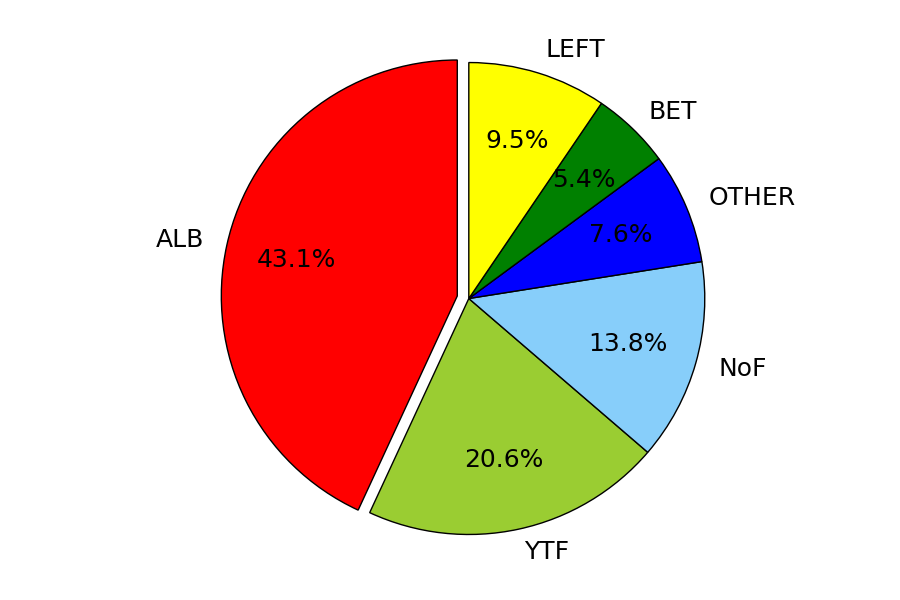
\includegraphics[width=0.45\linewidth]{figures/train_data.png}}
  \hspace{0.05in}
\subfigure[Valing database]{
  \label{fig:b}
  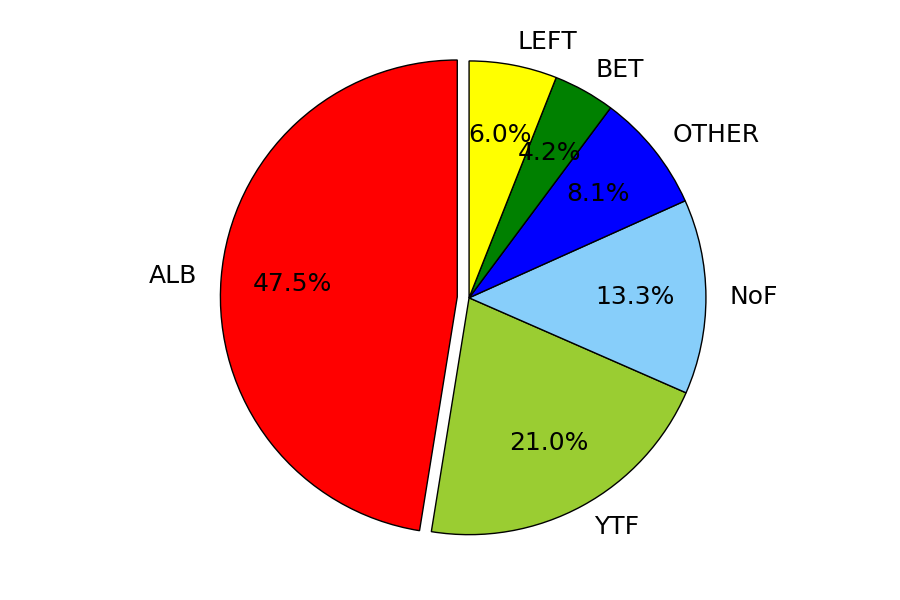
\includegraphics[width=0.45\linewidth]{figures/val_data.png}}
  \hspace{0.05in}
  \caption{Data distribution of Kaggle}
  \label{fig:data}

\end{figure}


% table
\begin{table}[t]
  \caption{singal model result on full data}
  \label{table:table2}
  \centering
  \begin{tabular}{lll}
    \toprule
    \cmidrule{1-3}
    database     &model       &accuracy \\
    \midrule
    full & alexnet     & 0.94 \\
    full & googlenet    &0.942 \\
    full  & vgg16    & 0.44 \\
    \bottomrule
  \end{tabular}
\end{table}


\begin{table}[t]
\small
\centering
\caption{Kaggle database}
\label{table:table3}
\begin{tabular}{lll}
    \toprule
    \cmidrule{1-3}
     database     &model      &accuracy \\
	\midrule
       full+rotating & alexnet     & 0.9673  \\
       full+rotating & googlenet   &0.964    \\
       full+rotating  & vgg16  & 0.45  \\
       \bottomrule
\end{tabular}
\end{table}

\begin{table}[t]
\small
\centering
\caption{Kaggle database}
\label{table:table4}
\begin{tabular}{lll}
    \toprule
    \cmidrule{1-3}
     database     &model        &accuracy \\
	\midrule
       full+rotating+mask & alexnet     & 0.9703  \\
       full+rotating+mask & googlenet   &0.954    \\
  
       \bottomrule
\end{tabular}
\end{table}



%The second method is to pick up some images to do image processing. We have made a mask of the area where the fish are located, and we used both the processed images and the raw images to train our model. Fig.~\ref{fig:mosaic} shows the differences between the two images. This method can force our neural network to concentrate on the area where the fish present. And the features are learned from comparing the raw images with the images with mask. In this method, We modified the Caffe\cite{jia2014caffe} to get the pooled image data to search the more significant area in classification. Through comparing the pooling gray image with the raw image, we found that the area of fish is brighter than other areas, which proves what we expected that the fish area make great contribution in the classification. Fig.~\ref{fig:pool} illustrates the image information of the region of fish and other regions without fish. We can see that the region of fish is brighter than other regions and the pooling image data can confirm that the learned features are from fish. In addition, we use the processed images to finetune our pre-trained model and it performs better when testing.\par


The second improvement is based on an image preprocessing method. In order to force the neural networks focusing on fish not the vessel, we have made a mask of the area where the fish are located, and we used both the processed images and the raw images to train our model. Fig.~\ref{fig:mosaic} shows the differences between the two images. This method can force our neural network to concentrate on the area where the fish present. And the features are learned from comparing the raw images with the images with mask. In order to prove our assumption, we test one fish image  and get the image data from the last pooling layer. The higher value area in the pooling layer means higher contribution to the final decision. Through comparing the pooling gray image with the raw image, we found that the area of fish is brighter than other areas, which proves what we expected that the fish area make great contribution in the classification. Fig.~\ref{fig:pool} illustrates the image information of the region of fish and other regions without fish. We can see that the region of fish is brighter than other regions and the pooling image data can confirm that the learned features are from fish. In addition, we use the processed images to fine-tune our pre-trained model and it performs better when testing.\par
The architecture of our model used in the experiment is the convolutional neural network(CNN), which has achieved remarkable performance in image classification and object detection recently. We employ the CNN architecture for the fish classification. But there still exists the problem that our model can not distinguish between foreground and background. Our methods can prevent the CNN architecture model from concentrating on the boat region rather than the fish region.

% mosaic pictures
\begin{figure}[!ht]
\centering

\subfigure[the raw image]{
  \label{fig:a}
  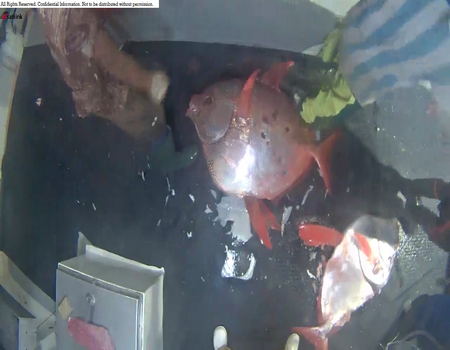
\includegraphics[width=0.45\linewidth]{figures/testout.png}}
  %\hspace{0.15in}
%\end{figure}
%\begin{figure}[!ht]
\subfigure[image with mask]{
  \label{fig:b}
  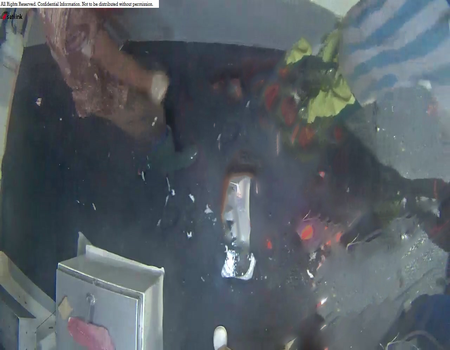
\includegraphics[width=0.45\linewidth]{figures/testout_raw.png}}
  %\hspace{0.15in}
  
  \caption{We make a mask of the area where the fish are located because the mask can force our model concentrate on the fish area. So it can help our convolutional nueral network detect the fish. we have trained our model useing both the two images at the same time, which can improve the robustness.}
   \label{fig:mosaic}

\end{figure}


%Recently, several papers have brought some methods for fish detection and classification\cite{chuang2016feature}. Spatial constraints are are introduced by dividing the image to regions and learning the feature region\cite{anantharajah2014local}. In order to divide the image to feature regions and background regions, We have made a mask in the fish region. And we use the mask images to lead our model to fit the feature regions and ignore the other regions.\cite{ge2015modelling} 

%the accuracy using rotating
%\par
%The architecture of our model used in the experiment is the convolutional neural network(CNN). And CNN is usually composed of convolutional layer, pooling layer and fully connected layer. CNN has achieved remarkable performance in image classification recently. Compared with feature-designed extraction, it can explore more abstract and high-level information by deep neural network. So we can apply it in fish classification. 











%THe rest of the paper is organised as follows. In section 2, we describe some related works about zooplankton classifition. Some basic introduction about the convolutional neural network and the details of the image calssification traning and evaluation are then presented in Section 3. Section 4 desribe that the experimental results of Zooplankton and the comparison with the performances of other methods in the dataset. Section 5 concludes the paper in the end. 
%\hfill mds
 
%\hfill January 11, 2007



%\section{Transfer reinforce model and Training}
%Fig.~\ref{fig:network} illustrates the final transfer reinforce model archicture. We take the whole data as the input of our model and fixed model A as a feature extracter as expected to reinforce the small class's features. 

%\subsection{Archicture}




%pooling image
\begin{figure}[!ht]

\centering
\subfigure[the image]{
  \label{fig:a}
  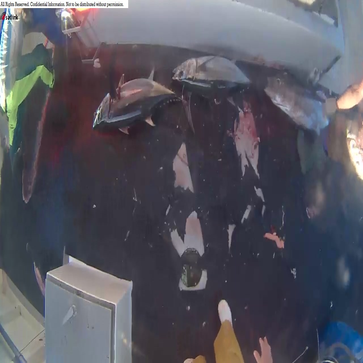
\includegraphics[width=0.45\linewidth]{figures/img.png}}
  \hspace{0.15in}
%\end{figure}
%\begin{figure}[!ht]
\subfigure[the pooling image]{
  \label{fig:b}
  
\includegraphics[width=0.45\linewidth]{figures/123.png}}
  \hspace{0.15in}
  \caption{The region of fish are brighter than other regions, which can prove that the fish has more influence on the classification.}
  \label{fig:pool}
\end{figure}


%\begin{figure*}[!ht]
%\centering
%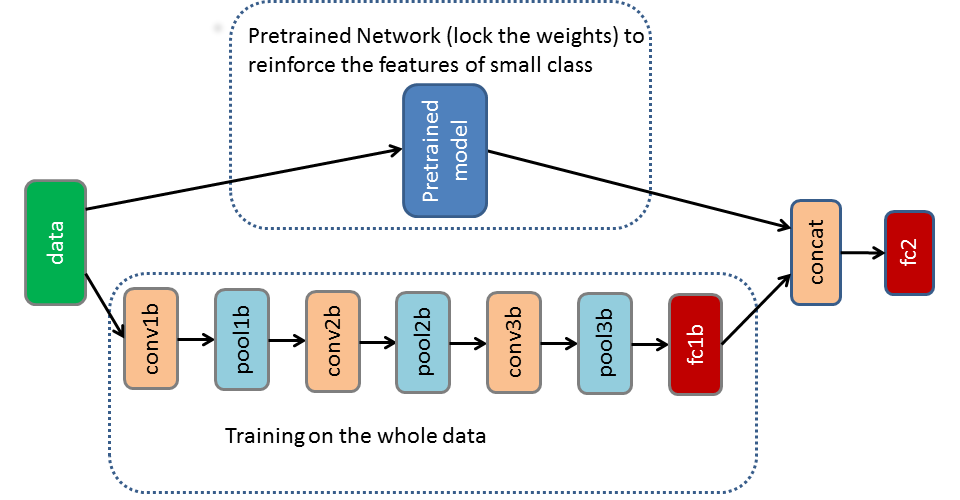
\includegraphics[width=0.85\textwidth]{figures/network.png}
%\caption{Model structure of our plankton classifaction neural network.}
%\label{fig:network}
%\end{figure*}

%\subsection{Training}


%\section{Experiments}
%Fig.~\ref{fig:a}, Fig.~\ref{fig:b}

\section{Experiments}
The Table~\ref{table:table1} indicates the details of the Kaggle Database. The first column is the name of fish and the numbers in the rest columns mean that the proportion of this class in all fish. And the Fig.~\ref{fig:data} is also the another form of fish proportion. We can see the distribution of the dataset is imbalanced. The Table~\ref{table:table2} illustrates the benchmarks. We can see the AlexNet and the GoogLeNet achieved greater performance than the VGGNet. The Table~\ref{table:table3} shows the accuracy that we have rotated some images to get new images. From the table we can see this method actually worked out and the accuracy has increased about two percent. Basing this, we have made a mask of the region of fish. The accuracy has also increased in the Table~\ref{table:table4}, which proves that our methods are effective.





\section{Conclusion}

%We have used two methods to help our model to detect the fish and avoid the over-fitting. We have done the data augmentation and found that it can improve the accuracy and help avoid over-fitting. And comparing the raw image and the mask image can help our model to detect the fish. We have used both the two methods simultaneously and the classification accuracy has increased more than two percent.
In this paper, we used two methods to improve deep neural networks to detect the fish more efficiently. The experiment results show that our methods can classify fish from images captured on a camera of fishing vessels well. And the classification accuracy has increased more than two percent.

% trigger a \newpage just before the given reference
% number - used to balance the columns on the last page
% adjust value as needed - may need to be readjusted if
% the document is modified later
%\IEEEtriggeratref{8}
% The "triggered" command can be changed if desired:
%\IEEEtriggercmd{\enlargethispage{-5in}}

% references section

% can use a bibliography generated by BibTeX as a .bbl file
% BibTeX documentation can be easily obtained at:
% http://www.ctan.org/tex-archive/biblio/bibtex/contrib/doc/
% The IEEEtran BibTeX style support page is at:
% http://www.michaelshell.org/tex/ieeetran/bibtex/
%\bibliographystyle{IEEEtran}
% argument is your BibTeX string definitions and bibliography database(s)
%\bibliography{IEEEabrv,../bib/paper}
%
% <OR> manually copy in the resultant .bbl file
% set second argument of \begin to the number of references
% (used to reserve space for the reference number labels box)
%\begin{thebibliography}{1}

%\bibitem{IEEEhowto:kopka}
%H.~Kopka and P.~W. Daly, \emph{A Guide to \LaTeX}, 3rd~ed.\hskip 1em plus
%  0.5em minus 0.4em\relax Harlow, England: Addison-Wesley, 1999.

%\end{thebibliography}
\bibliographystyle{IEEEtran}
\bibliography{test}


% that's all folks
\end{document}


